\chapter{Solution approach}

% ~~~~~~~~~~~~~~~~~~~~~~~~~~~~~~~~~~~~~~~~~~~~~~~~~~~~~~~~~~~~~~~~~~~~~~~~~~~~~~~~~~~~~~~~~~~~~~~~~~~~~~~~~~~
\section{Baseline solution}

\begin{itemize}
    \item Adapt existing simple indicators to detect bottlenecks

    \item \TODO{Adaptations of existing indicators}    

    \item Try to find alternative schedule based on the found bottlenecks
    \begin{itemize}
        \item Combinatorial heuristics?
        \item Simplified optimization?
    \end{itemize}
\end{itemize}

\begin{figure}[p]\centering
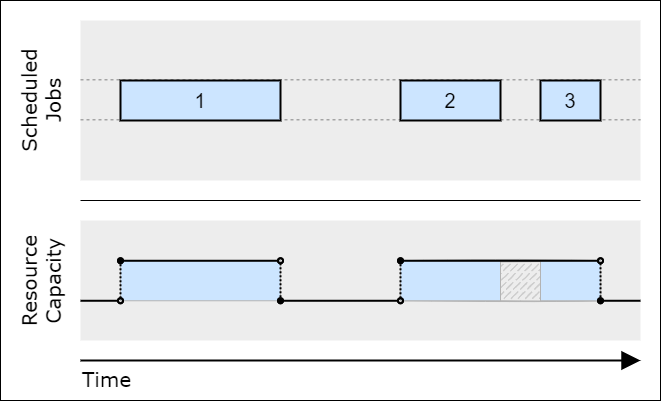
\includegraphics[width=\textwidth]{img/Capacities-JobShop.png}
% Příponu není potřeba explicitně uvádět, pdflatex automaticky hledá pdf.
% Rozměry také není nutné uvádět.
\caption{Caption}
% \label{Label}
\end{figure}

% ~~~~~~~~~~~~~~~~~~~~~~~~~~~~~~~~~~~~~~~~~~~~~~~~~~~~~~~~~~~~~~~~~~~~~~~~~~~~~~~~~~~~~~~~~~~~~~~~~~~~~~~~~~~
\section{Extended solution}

\begin{itemize}
    \item Come up with a new way of detecting time-variant bottlenecks
    \item Apply the method to identify bottlenecks
    \item Relax bottlenecks - one by one, combined?
    \item Propose alternative solutions
    \begin{itemize}
        \item Extremal solutions based on some similarity/improvement metrics?
        \item Scalable solution?
    \end{itemize}
\end{itemize}
